\chapter{Estudio previo}\label{cap:planificación}

\section{Introducción}

En este capítulo se presenta el estudio previo realizado para el desarrollo del sistema \textbf{Sevillaneando}. Este análisis tiene como finalidad definir el contexto del proyecto, establecer los objetivos principales, seleccionar la metodología de trabajo más adecuada junto la planificación de las distintas fases del proyecto.

El estudio previo constituye una base fundamental para el resto del proyecto, ya que permite organizar el trabajo de manera estructurada, analizar las tecnologías más apropiadas y estimar los recursos necesarios. Asimismo, facilita la toma de decisiones durante el desarrollo y asegura la coherencia entre los requisitos iniciales y la solución final implementada.

\section{Objetivos}

\subsection{Objetivos del proyecto}

Los objetivos del proyecto son aquellos que persigue la estudiante como futura ingeniera de software en el marco del Trabajo de Fin de Grado:

\begin{itemize}
    \item Aplicar en un contexto real los conocimientos adquiridos a lo largo del Grado en Ingeniería del Software, especialmente en las áreas de diseño de software, arquitecturas de sistemas, ingeniería de requisitos y gestión de proyectos.

    \item Desarrollar la capacidad de planificación, seguimiento y autogestión en un proyecto de desarrollo unipersonal, adoptando un proceso iterativo e incremental basado en metodologías ágiles.

    \item Adquirir experiencia práctica en tecnologías modernas de desarrollo web y móvil (React Native, NestJS, PostgreSQL/PostGIS, Firebase) que complementen la formación académica con competencias técnicas de industria.

    \item Adentrarse por primera vez en el desarrollo de aplicaciones móviles, un ámbito no cubierto durante el Grado, afrontando sus particularidades: ciclo de vida de la aplicación, adaptación a múltiples plataformas (iOS y Android) y compilación y distribución mediante Expo.

    \item Consolidar el uso de TypeScript en un proyecto complejo de extremo a extremo, profundizando en el tipado estático y en las buenas prácticas del lenguaje más allá del contacto puntual previo, aplicándolo tanto en el frontend (React Native) como en el backend (NestJS).

    \item Enfrentar y resolver retos técnicos no triviales: comunicación bidireccional en tiempo real, consultas geoespaciales, scraping automatizado y diseño de un motor de recomendaciones.

    \item Producir documentación técnica de calidad (memoria, manuales de usuario, de desarrollo y de despliegue) como parte de las entregas propias de un proyecto profesional.
\end{itemize}

\subsection{Objetivos del sistema}

El objetivo principal del sistema es el desarrollo de una aplicación móvil orientada al descubrimiento de eventos y actividades en Sevilla, con especial énfasis en dar visibilidad a eventos emergentes o poco conocidos.

A partir de este objetivo general, se definen los siguientes objetivos específicos del sistema:

\begin{itemize}
    \item Diseñar e implementar un sistema que permita listar eventos con información detallada (descripción, ubicación, imágenes, precio, etc.) y filtrado de eventos.

    \item Permitir a los usuarios crear nuevos eventos, diferenciando entre eventos públicos y privados, e incorporando un sistema de moderación para garantizar la fiabilidad de los eventos públicos.

    \item Permitir a los usuarios editar los eventos creados por sí mismos.

    \item Integrar funcionalidades de geolocalización para mostrar eventos cercanos y permitir su visualización en un mapa interactivo para un acceso más cómodo.

    \item Promover la interacción social entre usuarios mediante chat en eventos, mensajería privada, seguimiento entre usuarios y opiniones en las valoraciones.

    \item Implementar un sistema de recomendaciones personalizado basado en la actividad del usuario (guardar un evento, apuntarse a un evento, compartir un evento, ver un evento, valorar un evento, etc.), sus intereses y su ubicación.

    \item Desarrollar un sistema de rutas recomendadas de eventos que permita agrupar actividades según gustos y criterios de proximidad y horario.

    \item Permitir a los usuarios crear rutas de eventos que sean visibles para el resto y que puedan valorarlas.

    \item Incluir notificaciones para informar al usuario sobre eventos cercanos, recordatorios, seguidores nuevos y aprobación o rechazo de los eventos.
\end{itemize}

\section{Metodología}

En este apartado se describe la metodología seguida durante el proyecto, organizada en tres ámbitos de actuación con distintos niveles de abstracción: la gestión general del proyecto, la gestión del proceso de desarrollo y la gestión del código fuente. Adicionalmente, se recoge la metodología de seguimiento del tiempo.

\subsection{Metodología de gestión del proyecto}

El desarrollo del proyecto se ha llevado a cabo mediante una adaptación de la metodología ágil Scrum, ajustada al contexto de un Trabajo de Fin de Grado.

Al tratarse de un equipo unipersonal, la desarrolladora ha asumido simultáneamente los roles de \textit{Product Owner}, \textit{Scrum Master} y desarrolladora. Esto ha permitido una toma de decisiones ágil, aunque también ha requerido una mayor disciplina en la autogestión del tiempo y las prioridades.

Dado que el proyecto ha sido desarrollado por un único miembro, no se han realizado reuniones diarias (\textit{daily stand-ups}). En su lugar, la comunicación se ha mantenido de forma continua mediante tutorías periódicas con el tutor académico. Estas sesiones han combinado la revisión del trabajo realizado con la planificación del siguiente sprint, permitiendo mantener una evolución iterativa del sistema y adaptar el alcance en función del tiempo disponible y de las prioridades del proyecto.

Para la gestión del backlog y el seguimiento de tareas se han utilizado \textbf{GitHub Projects} como tablero Kanban, complementado con un documento Word donde se ha mantenido el backlog detallado junto con las actas de reunión de cada tutoría, en las que se recogen las tareas completadas en el sprint anterior y los objetivos definidos para el siguiente.

\subsection{Metodología de gestión del desarrollo}

La estimación de tareas se ha realizado mediante la técnica de tallas de camiseta (\textit{T-shirt sizing}), que asigna un tamaño relativo a cada historia: XS (extra pequeña), S (pequeña), M (mediana), L (grande) y XL (extra grande). La talla se define en función de la complejidad, el riesgo y la cantidad de trabajo, comparando cada historia con otras ya conocidas. Esta estimación permite priorizar el backlog combinando valor (prioridad) y esfuerzo (talla), facilitando la planificación ágil y la selección de historias por sprint.

Adicionalmente, se ha configurado un pipeline de integración y entrega continua (CI/CD) mediante \textbf{GitHub Actions}, que automatiza los despliegues y la ejecución del linter y las comprobaciones de formato en cada push, contribuyendo a mantener la calidad del código a lo largo del desarrollo.

\subsection{Metodología de gestión del código fuente}

Para la gestión del código fuente se ha utilizado un sistema de control de versiones Git, permitiendo mantener el historial de cambios y asegurando el orden y la claridad en el desarrollo.

Se ha seguido una política de ramas sencilla basada en \textit{main}, para la versión estable; \textit{develop}, para la integración de nuevas funcionalidades antes de fusionarlas en \textit{main}; y ramas de funcionalidad (\textit{feature/*}), derivadas de \textit{develop}.

Además, se ha aplicado el estándar \textit{Conventional Commits} para mantener un historial de cambios claro y estructurado, siguiendo la siguiente convención:

\begin{center}
\texttt{<tipo> [alcance opcional]: <descripción corta>}
\end{center}

Los tipos utilizados han sido:

\begin{itemize}
    \item feat: Nueva funcionalidad.
    \item fix: Corrección de errores.
    \item docs: Cambios en la documentación.
    \item style: Ajustes de formato sin afectar a la funcionalidad.
    \item refactor: Cambios en el código sin alterar la funcionalidad.
    \item test: Añadir o modificar pruebas.
    \item chore: Tareas de mantenimiento o configuración.
\end{itemize}

También se ha seguido un versionado semántico de tres niveles (X.Y.Z) para la política de versiones del software:

\begin{itemize}
    \item X: Versión mayor, ante cambios incompatibles o rediseños importantes.
    \item Y: Versión menor, al añadir nuevas funcionalidades.
    \item Z: Versión de parche, para corregir errores o problemas menores.
\end{itemize}

\subsection{Metodología de seguimiento del tiempo}

El seguimiento del tiempo dedicado al proyecto se ha realizado con la herramienta \textbf{Clockify}, lo que ha permitido monitorizar el esfuerzo real invertido en cada fase y mantener la coherencia entre la planificación estimada y el trabajo efectivamente realizado. El informe detallado de horas se recoge en el Anexo correspondiente.

\section{Planificación}

La planificación del proyecto se ha estructurado en varias fases, siguiendo un enfoque incremental:

\begin{itemize}
    \item \textbf{Fase 0 – Determinación del alcance}: definición del alcance funcional del sistema, identificación del problema a resolver, análisis del contexto y de las soluciones existentes, y establecimiento de las restricciones y criterios de éxito del proyecto.

    \item \textbf{Fase 1 – Análisis y planificación}: definición de requisitos y alcance, elaboración del backlog inicial, planificación temporal y de recursos (cronograma inicial) y diseño del modelo conceptual del sistema.

    \item \textbf{Fase 2 – Diseño}: diseño de la arquitectura técnica, de la interfaz de usuario, de la base de datos, de la API REST y planificación de la gestión de usuarios y permisos.

    \item \textbf{Fase 3 – Desarrollo}: implementación del sistema, incluyendo el frontend móvil (React Native + Expo) y el backend (NestJS), así como funcionalidades como eventos, chat, mapa, notificaciones y recomendaciones.

    \item \textbf{Fase 4 – Pruebas y validación}: ejecución de pruebas funcionales, de integración y de usabilidad, así como la corrección de errores.

    \item \textbf{Fase 5 – Ampliaciones y extras}: funcionalidades adicionales condicionadas al tiempo disponible, como la generación de carteles con IA, la gestión de calendarios y el filtrado de contenido inapropiado (NSFW).

    \item \textbf{Fase 6 – Despliegue y cierre del proyecto}: despliegue del sistema, elaboración de la memoria técnica y los manuales, creación de los materiales de defensa del proyecto y cierre formal del trabajo.
\end{itemize}

\subsection{Desviaciones respecto a la planificación inicial}

A lo largo del proyecto se han producido algunas desviaciones respecto a la planificación inicial, motivadas principalmente por la aparición de nuevas necesidades técnicas y por el ajuste del alcance en función del tiempo disponible.

\begin{itemize}
    \item \textbf{Incorporación de flujos de CI/CD} \textit{(Fase 6 – Sprint 6)}: inicialmente no estaba prevista la configuración de pipelines de integración continua. Sin embargo, durante el Sprint 6 se consideró conveniente automatizar las comprobaciones de calidad del código mediante GitHub Actions. La configuración del pipeline, incluyendo la integración del linter, las comprobaciones de formato y los flujos de despliegue, supuso una dedicación de aproximadamente 6 horas, no contempladas en la estimación original de cierre del proyecto.

    \item \textbf{No implementación de funcionalidades opcionales} \textit{(Fase 5)}: la Fase 5 del proyecto (ampliaciones y extras) estaba condicionada a la disponibilidad de tiempo una vez completadas las fases principales. Finalmente, la generación de carteles con IA y la moderación automática de imágenes mediante NSFWJS no pudieron implementarse, ya que el desarrollo de las funcionalidades core del sistema (especialmente rutas de eventos, sistema de recomendaciones y scraping) requirió más esfuerzo del estimado inicialmente.

    \item \textbf{Mayor complejidad en el scraping} \textit{(Fase 3 – Sprint 4)}: la integración del motor de scraping implicó una complejidad técnica superior a la prevista. Se estimaban entre 10 y 15 horas de desarrollo, pero el trabajo real ascendió a aproximadamente 20--22 horas. La desviación se debió principalmente a la gestión de errores 429 (límite de peticiones) y la variabilidad en la estructura de las fuentes externas, lo que requirió iteraciones adicionales de corrección y ajuste. A ello se sumaron tres dificultades no previstas: en primer lugar, la clasificación de los eventos extraídos en las categorías existentes del sistema resultó especialmente laboriosa, ya que los títulos y descripciones de las fuentes externas no siguen ninguna taxonomía estándar; fue necesario diseñar y refinar iterativamente una lista de palabras clave por categoría hasta lograr una asignación razonablemente precisa. En segundo lugar, la extracción de direcciones reales presentó dificultades por la falta de uniformidad en cómo cada fuente representa la ubicación, mezclando nombres de recintos, barrios, referencias parciales y formatos libres. En tercer lugar, el tratamiento de fechas supuso un reto significativo: muchas fuentes presentan sus calendarios de eventos en formatos no lineales (calendarios visuales, rangos de fechas, sesiones múltiples), lo que obligó a reajustar en varias ocasiones la lógica de extracción y normalización de fechas para cubrir los distintos casos encontrados.

    \item \textbf{Impacto de las fechas del scraping en el sistema de rutas} \textit{(Fase 3 – Sprint 5)}: los problemas de normalización de fechas descritos en el punto anterior tuvieron también un efecto directo sobre el sistema de rutas recomendadas, cuyo desarrollo se concentró en el Sprint 5. Las rutas agrupan eventos por fecha como criterio de organización, por lo que los eventos del scraping que presentaban un calendario de fechas múltiples o indeterminadas no podían tratarse del mismo modo que los eventos con fecha única. Como solución, se decidió que cuando un evento procedente del scraping viene asociado a un calendario de sesiones, la fecha deja de usarse como factor de puntuación en la construcción de la ruta; en su lugar, se indica que existen varias fechas disponibles y el criterio de ordenación pasa a ser principalmente la distancia entre eventos. Fue necesario adaptar la lógica del algoritmo para detectar este caso y aplicar la estrategia adecuada. Esta incidencia supuso una desviación de aproximadamente 4--5 horas adicionales sobre las 12--14 horas estimadas para el algoritmo de rutas.

    \item \textbf{Problemas de compatibilidad con Android} \textit{(Fases 5 y 6 – Sprints 5 y 6)}: durante la fase de pruebas con usuarios piloto, llevada a cabo en el Sprint 5, se detectaron incidencias significativas en dispositivos Android que no habían aparecido durante el desarrollo, realizado íntegramente sobre iOS. Los principales problemas fueron la no visualización del mapa (OpenStreetMap) en Android y varios descuadres en la disposición de elementos de pantalla. La corrección de estas incidencias se extendió hasta el Sprint 6 y supuso una dedicación adicional de aproximadamente 7--8 horas no previstas en la planificación original. Esta desviación pone de manifiesto la importancia de incorporar pruebas sobre ambas plataformas desde las primeras fases del desarrollo.
\end{itemize}

En términos generales, el proyecto se ha completado dentro del plazo establecido y con el alcance funcional definido como prioritario, asumiendo las desviaciones anteriores como decisiones justificadas de gestión del alcance. El esfuerzo total registrado ha sido de aproximadamente 300 horas de trabajo, distribuidas a lo largo de 29 semanas de desarrollo, lo que supone una media de algo más de 10 horas semanales. El detalle del registro de horas por fase y actividad se recoge en el informe de Clockify incluido como Anexo.

\subsection{Estructura de Desglose del Trabajo inicial}

La planificación inicial del proyecto se ha definido mediante una Estructura de Desglose del Trabajo (EDT), organizando el proyecto en fases, tareas y subtareas principales.

\begin{itemize}
    \item \textbf{Nivel 1: Proyecto ``Sevillaneando''}

    \item \textbf{Fase 0 -- Determinación del alcance}
    \begin{itemize}
        \item \textbf{0.1} Análisis del problema y contexto.
        \item \textbf{0.2} Estudio de soluciones existentes.
        \item \textbf{0.3} Definición del alcance funcional y restricciones del proyecto.
    \end{itemize}

    \item \textbf{Fase 1 -- Análisis y planificación}
    \begin{itemize}
        \item \textbf{1.1} Revisión de requisitos y alcance.
        \item \textbf{1.2} Elaboración del backlog inicial.
        \item \textbf{1.3} Planificación temporal y de recursos (cronograma inicial).
        \item \textbf{1.4} Creación del modelo conceptual.
    \end{itemize}

    \item \textbf{Fase 2 -- Diseño}
    \begin{itemize}
        \item \textbf{2.1} Diseño de arquitectura técnica.
        \item \textbf{2.2} Diseño de la interfaz (navegación, usabilidad).
        \item \textbf{2.3} Diseño de la base de datos (PostgreSQL + PostGIS).
        \item \textbf{2.4} Diseño de la API REST (endpoints principales).
        \item \textbf{2.5} Planificación de la gestión de usuarios y permisos.
    \end{itemize}

    \item \textbf{Fase 3 -- Desarrollo paralelo (Frontend y Backend)}

    \begin{itemize}
        \item \textbf{Fase 3A -- Desarrollo del frontend (React Native)}
        \begin{itemize}
            \item \textbf{3A.1} Configuración del entorno móvil (dependencias, entornos, etc.).
            \item \textbf{3A.2} Implementación del listado y detalle de eventos.
            \item \textbf{3A.3} Creación y moderación de eventos, categorías y usuarios.
            \item \textbf{3A.4} Integración del mapa (OpenStreetMap).
            \item \textbf{3A.5} Integración de búsqueda.
            \item \textbf{3A.6} Sistema de notificaciones.
            \item \textbf{3A.7} Integración de chat.
            \item \textbf{3A.8} Módulo de subida de fotos.
            \item \textbf{3A.9} Implementación de reseñas y valoraciones.
            \item \textbf{3A.10} Personalización de recomendaciones.
        \end{itemize}

        \item \textbf{Fase 3B -- Desarrollo del backend (Node.js + NestJS)}
        \begin{itemize}
            \item \textbf{3B.1} Configuración del servidor, base de datos e integración de autenticación.
            \item \textbf{3B.2} Implementación de endpoints de eventos, usuarios y categorías (CRUD, lógica de eventos privados y sistema de moderación).
            \item \textbf{3B.3} Sistema de notificaciones.
            \item \textbf{3B.4} Infraestructura de chat: WebSockets para chat.
            \item \textbf{3B.5} Integración de imágenes mediante Cloudinary.
            \item \textbf{3B.6} Motor de scraping: implementación de scrapers para captura periódica de eventos externos.
            \item \textbf{3B.7} Algoritmo de recomendaciones: lógica de filtrado colaborativo o basado en etiquetas para rutas e intereses.
        \end{itemize}
    \end{itemize}

    \item \textbf{Fase 4 -- Pruebas y validación}
    \begin{itemize}
        \item \textbf{4.1} Pruebas unitarias (de backend).
        \item \textbf{4.2} Pruebas de integración (API + app).
        \item \textbf{4.3} Pruebas de usabilidad con usuarios reales.
        \item \textbf{4.4} Corrección de errores y mejoras.
    \end{itemize}

    \item \textbf{Fase 5 -- Ampliaciones y extras}

    Esta fase se ejecutará únicamente si el cronograma de las fases anteriores lo permite.

    \begin{itemize}
        \item \textbf{5.1} Generación de carteles con IA.
        \item \textbf{5.2} Gestión de calendarios. \textit{(Implementado.)}
        \item \textbf{5.3} Filtrado de contenido inapropiado (NSFW) en imágenes subidas por los usuarios.
    \end{itemize}

    \item \textbf{Fase 6 -- Despliegue y cierre del proyecto}
    \begin{itemize}
        \item \textbf{6.1} Despliegue de backend y frontend.
        \item \textbf{6.2} Publicación de la app. \textit{(No realizado: la publicación en las tiendas oficiales (Google Play Store y App Store) requiere el pago de una tarifa de desarrollador, lo que queda fuera del alcance de este proyecto.)}
        \item \textbf{6.3} Elaboración de la memoria técnica y manuales de usuario, de despliegue y de desarrollo.
        \item \textbf{6.4} Preparación de los materiales de defensa del proyecto (presentación y vídeo demostrativo).
    \end{itemize}
\end{itemize}

\begin{figure}[H]
    \centering
    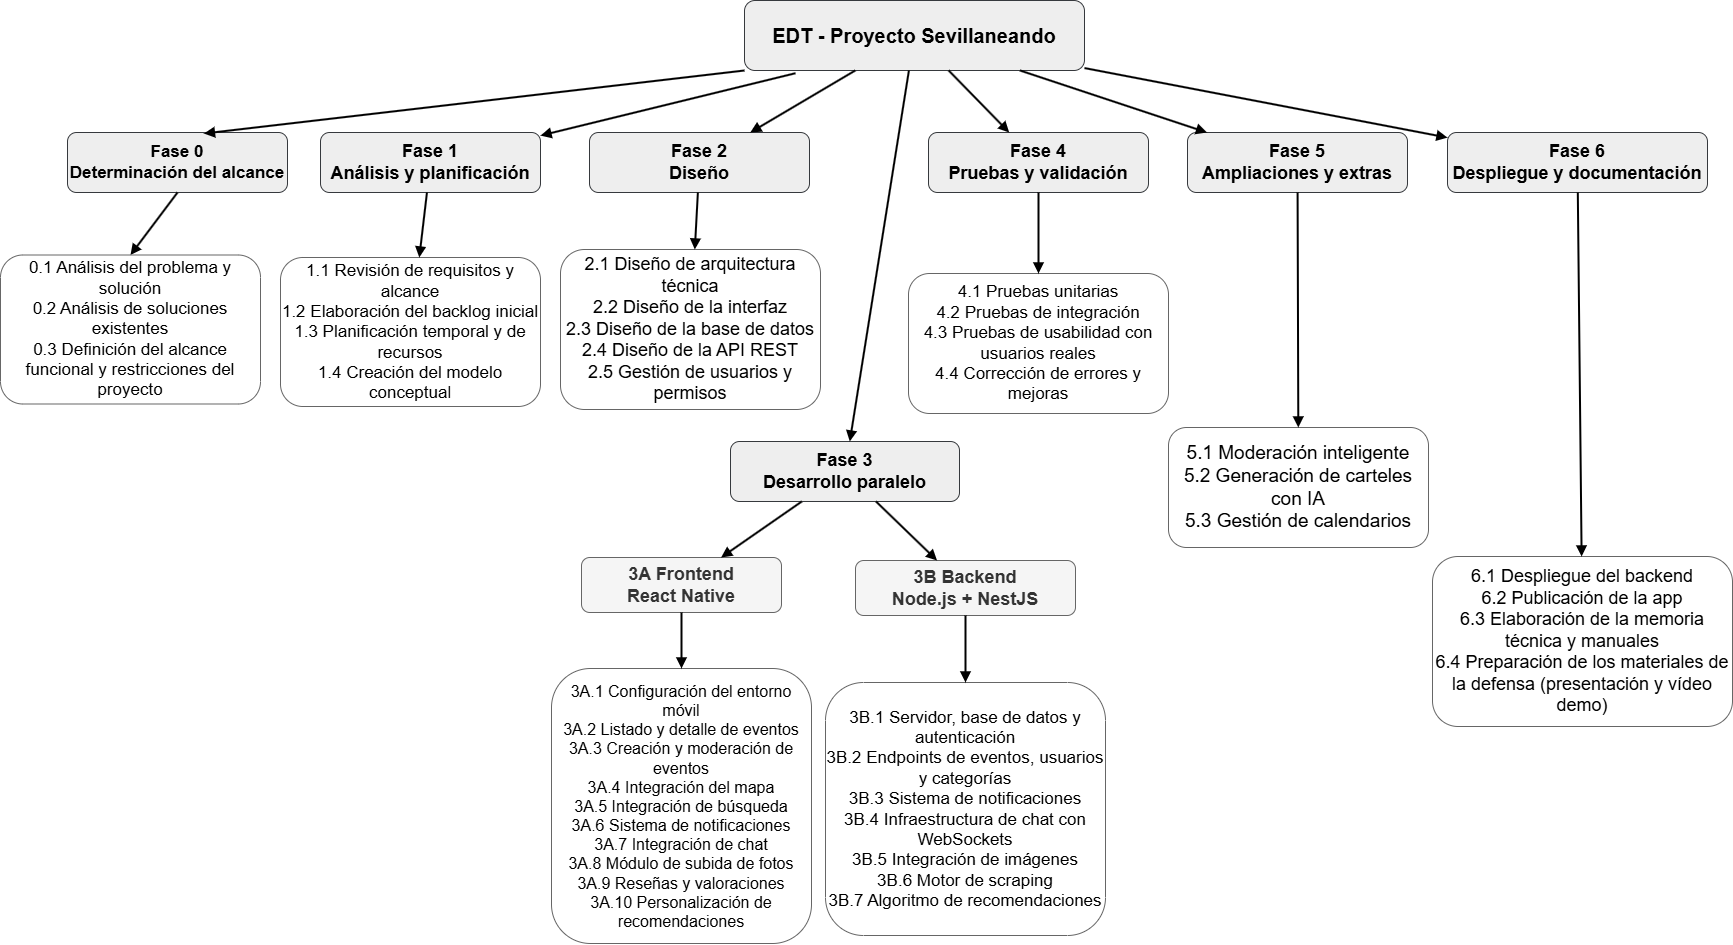
\includegraphics[width=1.1\textwidth]{figures/edt.png}
    \caption{Estructura de Desglose del Trabajo del proyecto}
    \label{fig:edt}
\end{figure}

\subsection{Planificación por sprints}

El desarrollo del proyecto se ha organizado en sprints de duración variable, adaptados a las necesidades del proyecto y a la disponibilidad temporal. En general, los sprints han tenido una duración aproximada de 4 semanas, ajustándose a 3 semanas en la fase final del proyecto.

\begin{longtable}{|p{2cm}|p{3cm}|p{4cm}|p{7cm}|}
\hline
\textbf{Sprint} & \textbf{Duración} & \textbf{Objetivo} & \textbf{Funcionalidades principales} \\
\hline
\endfirsthead

\hline
\textbf{Sprint} & \textbf{Duración} & \textbf{Objetivo} & \textbf{Funcionalidades principales} \\
\hline
\endhead

Sprint 1 & 4 semanas & MVP inicial & Sistema de autenticación, modelo conceptual, visualización básica de mapa \\
\hline

Sprint 2 & 4 semanas & Gestión de eventos & Creación y moderación de eventos, categorías, visualización en mapa, notificaciones \\
\hline

Sprint 3 & 4 semanas & Funcionalidades sociales & Chat en tiempo real (WebSockets), subida de imágenes, mejoras en búsqueda y filtrado geográfico \\
\hline

Sprint 4 & 4 semanas & Ampliación funcional & Scraping de eventos externos, gestión avanzada de imágenes, sistema de precios, optimización de chat \\
\hline

Sprint 5 & 3 semanas & Funcionalidad principal & Implementación del sistema de rutas de eventos y mejoras finales \\
\hline

Sprint 6 & 3 semanas & Cierre del proyecto & Refactorización, testing, validación, documentación y elaboración de la memoria \\
\hline

\end{longtable}

\subsection{Diagrama de planificación}

A continuación, se presenta un diagrama de Gantt simplificado que refleja la planificación temporal del proyecto, ajustada a la duración real de los sprints:

\begin{center}
\resizebox{\textwidth}{!}{%
\begin{ganttchart}[
    y unit title=0.5cm,
    y unit chart=0.6cm,
    vgrid,
    hgrid,
    bar height=0.35,
    title height=1,
    group right shift=0,
    group top shift=0.7
]{1}{29}

\gantttitle{Planificación del proyecto (semanas)}{29} \\
\gantttitlelist{1,...,29}{1} \\

\ganttbar{Análisis y planificación}{1}{3} \\
\ganttbar{Diseño}{4}{6} \\
\ganttbar{Sprint 1 (MVP)}{7}{10} \\
\ganttbar{Sprint 2 (Eventos)}{11}{14} \\
\ganttbar{Sprint 3 (Social)}{15}{18} \\
\ganttbar{Sprint 4 (Ampliaciones)}{19}{22} \\
\ganttbar{Sprint 5 (Rutas)}{23}{25} \\
\ganttbar{Sprint 6 (Cierre)}{26}{28} \\

\end{ganttchart}%
}
\end{center}

\section{Presupuesto}

El proyecto ha sido desarrollado en un contexto académico, por lo que no ha requerido una inversión económica directa significativa. No obstante, es posible realizar una estimación del coste real que tendría el proyecto si fuera encargado a una empresa de desarrollo de software, siguiendo la estructura estándar de presupuestación de proyectos informáticos.

\subsection{Recursos humanos}

El desarrollo ha sido llevado a cabo por una única persona asumiendo todos los roles del equipo. El coste unitario se estima a partir de las tablas salariales oficiales de referencia para el sector TIC en España, considerando un perfil de \textbf{Analista-Programadora junior}:

\begin{itemize}
    \item Coste hora base: \textbf{25 €/h}
    \item Total de horas: \textbf{300 h}
    \item Coste base de personal: 300 h $\times$ 25 €/h = \textbf{7.500 €}
\end{itemize}

Sobre el coste base de personal se aplican los \textbf{costes sociales} a cargo de la empresa (Seguridad Social, formación, contingencias), estimados en un 30\% del coste base:

\begin{itemize}
    \item Costes sociales: 7.500 € $\times$ 30\% = \textbf{2.250 €}
    \item Coste total de personal (base + sociales): \textbf{9.750 €}
\end{itemize}

\subsection{Distribución del esfuerzo}

El esfuerzo total del proyecto se ha estimado en aproximadamente 300 horas de trabajo. Esta distribución no es uniforme, ya que la mayor parte del esfuerzo se ha concentrado en el desarrollo frontend y backend.

\begin{longtable}{|p{6cm}|p{4cm}|}
\hline
\textbf{Fase} & \textbf{Horas estimadas} \\
\hline
Análisis y planificación & 25 h \\
\hline
Diseño del sistema & 30 h \\
\hline
Desarrollo frontend & 65 h \\
\hline
Desarrollo backend & 80 h \\
\hline
Refactorización y ajustes finales & 20 h \\
\hline
Testing y validación & 25 h \\
\hline
Despliegue & 15 h \\
\hline
Documentación y memoria & 60 h \\
\hline
\textbf{Total} & \textbf{300 h} \\
\hline
\end{longtable}

\subsection{Infraestructura y costes indirectos}

Para el desarrollo del proyecto han sido necesarios los siguientes recursos materiales e infraestructura, cuyos costes se imputan mediante amortización durante la vida útil estimada:

\begin{longtable}{|p{5cm}|p{2.5cm}|p{2cm}|p{2.5cm}|p{2.5cm}|}
\hline
\textbf{Recurso} & \textbf{Coste total} & \textbf{Vida útil} & \textbf{Duración proyecto} & \textbf{Coste imputable} \\
\hline
Ordenador portátil & 900 € & 4 años & 7 meses & 131 € \\
\hline
Conexión a internet & 40 €/mes & — & 7 meses & 280 € \\
\hline
Licencias y software & 0 € & — & — & 0 € \\
\hline
Herramientas en la nube (plan gratuito: Render, Supabase, Cloudinary, Firebase, GitHub) & 0 € & — & — & 0 € \\
\hline
\textbf{Total costes indirectos} & & & & \textbf{411 €} \\
\hline
\end{longtable}

\subsection{Coste total del proyecto}

\begin{longtable}{|p{8cm}|p{4cm}|}
\hline
\textbf{Concepto} & \textbf{Importe} \\
\hline
Coste de personal (base) & 7.500 € \\
\hline
Costes sociales (30\%) & 2.250 € \\
\hline
Costes indirectos (infraestructura) & 411 € \\
\hline
\textbf{Coste total del proyecto} & \textbf{10.161 €} \\
\hline
\end{longtable}

\subsection{Presupuesto}

El presupuesto es la cantidad que se cobraría al cliente por la realización del proyecto. A los costes totales se suman dos partidas adicionales:

\begin{itemize}
    \item \textbf{Margen de contingencia (12\%)}: cubre desviaciones razonables respecto a la estimación inicial. 10.161 € $\times$ 12\% = 1.219 €
    \item \textbf{Beneficio industrial (20\%)}: margen de beneficio habitual en el sector para proyectos de desarrollo de software. (10.161 € + 1.219 €) $\times$ 20\% = 2.276 €
\end{itemize}

\begin{longtable}{|p{8cm}|p{4cm}|}
\hline
\textbf{Concepto} & \textbf{Importe} \\
\hline
Coste total del proyecto & 10.161 € \\
\hline
Margen de contingencia (12\%) & 1.219 € \\
\hline
Beneficio industrial (20\%) & 2.276 € \\
\hline
\textbf{Presupuesto total (sin IVA)} & \textbf{13.656 €} \\
\hline
\textbf{IVA (21\%)} & \textbf{2.868 €} \\
\hline
\textbf{Presupuesto total (con IVA)} & \textbf{16.524 €} \\
\hline
\end{longtable}

Este presupuesto representa el valor de mercado del trabajo realizado. En el contexto del TFG no ha supuesto un gasto económico real, ya que las herramientas y servicios utilizados están disponibles en planes gratuitos y el trabajo ha sido realizado por la propia estudiante.
